\documentclass[alsotrans]{beamerswitch}
\usepackage{sdp}

\title{Списък}

% флаг дали да се включват слайдовете за CRTP
\def\crtp{article}
%\def\crtp{all}

\date[28.10--2.12.2019 г.]{28 октомври -- 2 декември 2019 г.}

\titlegraphicx{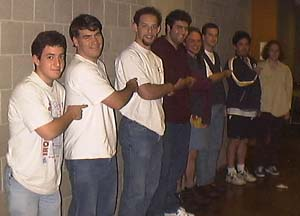
\includegraphics[height=0.25\textheight]{images/list.jpg}\\
  \imageUntitledAttr{Prettysleepy2}{https://pixabay.com/images/id-3517582/}{Pixabay License}}

% едносвързана верига
\newcommand{\linkedchain}{
  % веригата
  \doublecell{a1}{a_1}
  \nextdoublecell{a2}{a_2}{a1}
  \nextdots{a2}
  \dotsnextdoublecell{an-1}{a_{n-1}}
  \nextdoublecell{an}{a_n}{an-1}
}

% двусвързана верига
\newcommand{\doublelinkedchain}{
  % веригата
  \triplecell{a1}{a_1}
  \nexttriplecell{a2}{a_2}{a1}
  \triplenextdots{a2}
  \dotsnexttriplecell{an}{a_n}
}

\begin{document}

\begin{frame}
  \titlepage
\end{frame}

\section{АТД списък}

\begin{frame}
  \frametitle{АТД: списък}

  Хомогенна линейна структура с последователен достъп до елементите\\[2ex]
  Операции:\\[1ex]
  \begin{itemize}
  \item \tt{create()} --- създаване на празен списък
  \item \tt{empty()} --- проверка за празен списък
  \item \tt{insert(x, p)} --- включване на елемент \tt x на дадена позиция \tt p
  \item \tt{delete(p)} --- изключване на елемент на дадена позиция \tt p
  \item \tt{get(p)} --- достъп до елемент на дадена позиция \tt p
  \end{itemize}
\end{frame}

\begin{frame}
  \frametitle{Едносвързано представяне}

  \begin{center}
    \begin{tikzpicture}
      \linkedchain
      \nullptr{annext}

      % указател към началото
      \pointerto{a1.south}{\tt{front}}{below}

      % указател към края
      \pointerto{an.south}{\tt{back}}{below}
    \end{tikzpicture}
  \end{center}
\end{frame}

\begin{frame}
  \frametitle{Едносвързано циклично представяне}

  \begin{center}
    \small
    \begin{tikzpicture}
      % веригата
      \linkedchain

      % обратен указател
      \draw[pointer] (annext.center) -| ++(3em,-2em)  -| ($(a1data.west) - (2em,0)$) |- (a1data.west);

      % указател към началото
      \pointerto{a1.south}{\tt{start}}{below}
    \end{tikzpicture}
  \end{center}
\end{frame}

\begin{frame}<1>[label=doublelinked]
  \frametitle{Двусвързано представяне}

  \begin{center}
    \begin{tikzpicture}
      \doublelinkedchain
      \nullptr{a1prev}
      \nullptr{annext}

      % указател към началото
      \pointerto{a1.south}{\tt{front}}{below}

      % указател към края
      \pointerto{an.south}{\tt{back}}{below}
    \end{tikzpicture}
  \end{center}
\end{frame}

\begin{frame}
  \frametitle{Двусвързано циклично представяне}

  \begin{center}
    \begin{tikzpicture}
      \doublelinkedchain

      % обратен указател
      \draw[pointer] ([yshift=-.8ex]annext.center) -| ++( 3em,-2em)
      -| ($([yshift=-.8ex]a1.west) - ( 2em,0)$) to  (\tikztostart -| a1.west);

      % преден указател
      \draw[pointer] ([yshift= .8ex]a1prev.center) -| ++(-3em, 2em)
      -| ($([yshift= .8ex]an.east) - (-2em,0)$) to (\tikztostart -| an.east);

      % указател към началото
      \pointerto{a1.south}{\tt{start}}{below}
    \end{tikzpicture}
  \end{center}
  % изкуствено повторение на слайда, за да няма предупреждения при againframe
\end{frame}

\section{Итератори}

\begin{frame}
  \frametitle{АТД итератор}

  Абстракция на позиция, позволяваща обхождането на данни в дадена колекция\\[2ex]
  Операции:\\[1ex]
  \begin{itemize}
  \item \tt{begin()} -- инициализация в началото на списъка
  \item \tt{end()} -- инициализация в края на списъка
  \item \tt{next()} -- преместване напред
  \item \tt{prev()} -- преместване назад
  \item \tt{get()} -- достъп до елемент на дадената позиция
  \item \tt{valid()} -- проверка за валидност
  \end{itemize}
\end{frame}

\begin{frame}
  \frametitle{Итератор: физическо представяне}

  \begin{itemize}
  \item при свързано представяне --- указател към двойна или тройна кутия
  \item при последователно представяне --- индекс на пореден елемент
  \end{itemize}
\end{frame}

\begin{frame}[fragile]
  \frametitle{Цикъл върху контейнери}
  В C++11 имаме възможност да итерираме по елементите в даден контейнер със следния синтаксис:\\
  \tta{for(}<тип> <елемент> \tta: <израз>\tta) <оператор>
  \pause
  \begin{itemize}[<+->]
  \item{} <израз> трябва да се оценява до контейнер
  \item{} <тип> трябва съвпада с типа на елементите в контейнера
  \item{} <оператор> е тялото на цикъла, в което може да се използва <eлемент>
  \item ако <тип> е препратка, то <елемент> може да се използва за промяна на стойността на съответната позиция в контейнера
  \end{itemize}
  \onslide<+->
  Превежда се до:
\begin{lstlisting}
@\textsf{<подходящ тип>}@ const& c = @\textsf{<израз>}@;
for(@\textsf{<подходящ тип>}@ it = c.begin(); it != c.end(); ++it) {
  @\textsf{<тип>}@ @\textsf{<елемент>}@ = *it;
  @\textsf{<оператор>}@
}
\end{lstlisting}
\end{frame}

\mode<\crtp>
\begin{frame}
  \frametitle{Достъп до производен клас на шаблон}

  \textbf{Проблем:} Какъв резултат трябва да връщат операциите \tt{++}, преместващи итераторите?\\[2ex]
  \begin{itemize}
  \item \lst{Iterator\& operator++();}
    \begin{itemize}
    \item връщаме псевдоним към обект от абстрактен клас, ОК
    \end{itemize}
  \item\lst{Iterator operator++(int);}
    \begin{itemize}
    \item връщаме обект от абстрактен клас, \alert{грешка!}
    \end{itemize}
  \end{itemize}
  \vspace{2ex}
  \pause
  Трябва абстрактният базов клас да знае кой е конкретния му наследник! Възможно ли е това?\\[2ex]
  \pause
  \alert{Да! Базовият клас трябва да е \textbf{шаблон, приемащ производния си клас за параметър}}
\end{frame}

\begin{frame}[fragile]
  \frametitle{Curiously Recurring Template Pattern (CRTP)}

\begin{lstlisting}
template <typename Derived>
class Base {
  ...
};

class Derived : public Base<Derived> {
  ...
};
\end{lstlisting}
  По този начин шаблонът \lst{Base} може да се обръща към наследяващия го клас.
\end{frame}

\begin{frame}[fragile]
  \frametitle{Решение на проблема с \lst{operator++}}

  \small
\begin{lstlisting}
template <typename T, @\alert{typename ConcreteIterator}@>
class Iterator {
  ...
  @\alert{ConcreteIterator}@ operator++(int) {
    ConcreteIterator save = (ConcreteIterator&)*this;
    ++(*this);
    return save;
  }
};
template <typename T>
class LinkedListIterator :
         public Iterator<T, @\alert{LinkedListIterator<T>}@ > {
  ...
};
\end{lstlisting}
\pause
Експлицитното преобразуване на типа се налага, понеже \lst{*this} е от тип \lst{Iterator&}, а конструкторът за копиране на \lst{ConcreteIterator} очаква тип \lst{ConcreteIterator&}.
\end{frame}

\mode
<all>

\begin{frame}<1-7| trans:3,6>
  \frametitle{\alt<all:1-3>{Включване}{Изключване} на елемент \alt<all:1-3>{в}{от} едносвързан списък}

  \begin{center}
    \begin{tikzpicture}
      \dotsnode
      \dotsnextdoublecell{ai}{a_i}
      \doublecell[right=4em of ai]{ai+1}{a_{i+1}}{ai}
      \draw[pointer,visible on=<{all:1-2,5-}>] (ainext.center) to (ai+1);
      \nextdots{ai+1}

      % указател към елемента след който вмъкваме
      \pointerto{ai.south}{\tt{it.ptr}}{below}

      \begin{scope}[visible on=<all:2-6>]
        \doublecell[above right=6ex of ai.north]{new}x
        \pointerto{new}{\tt p}{above}
        \draw[pointer] (newnext.center) to (ai+1);
      \end{scope}

      \draw[pointer,visible on=<all:3-4>] (ainext.center) to (new);

      \draw (new) node[cross,visible on=<all:6>] {};
    \end{tikzpicture}
  \end{center}
\end{frame}

\begin{frame}
  \frametitle{Сложност на операции за едносвързан списък}
  Бързи операции (сложност $O(1)$ по време и памет):
  \begin{itemize}
  \item \tt{insertAfter}
  \item \tt{deleteAfter}
  \item \tt{insertFirst}
  \item \tt{insertLast}
  \item \tt{deleteFirst}
  \end{itemize}
  \pause
  Бавни операции (сложност $O(n)$ по време и $O(1)$ по памет):
  \begin{itemize}
  \item \tt{insertBefore}
  \item \tt{deleteLast}
  \item \tt{deleteAt}
  \item \tt{deleteBefore}
  \end{itemize}
\end{frame}

\begin{frame}
  \frametitle{Гранични случаи}
  Случаи, които изискват особено внимание:
  \begin{itemize}[<+->]
  \item Включване на елемент в празен списък
  \item Включване на елемент преди първия
  \item Включване на елемент след последния
  \item Изключване на единствения елемент на списък
  \item Изключване на първия елемент
  \item Изключване на последния елемент
  \item Опит за изключване на елемент от празен списък
  \item Опит за изключване преди първия елемент
  \item Опит за изключване след последния елемент
  \end{itemize}
\end{frame}

\section{Приложения на списъци}

\begin{frame}
  \frametitle{Задачи за списъци}

  \textbf{Задача.} Да се залепи на края на даден списък втори даден списък.\\[2ex]
  \pause
  \textbf{Решение №1 (абстрактно):} \visible<4->{\alert{O(n)}}\\
  Добавяме елементите на втория списък на края на първия.\\[2ex]
  \pause
  \textbf{Решение №2 (конкретно):} \visible<4->{\alert{O(1)}}\\
  Завързваме началото на втория списък за края на първия.\\[2ex]
  \pause\pause
  \textbf{Задача.} Да се обърне реда на елементите в даден списък.\\[2ex]
  \pause
  \textbf{Решение №1 (абстрактно):}\\
  Преместваме последователно елементите след първия елемент на списъка в началото на списъка.\\[2ex]
  \pause
  \textbf{Решение №2 (конкретно):}\\
  Разместване на указателите ``на място''.
\end{frame}

% TODO: анимация за mergesort с TikZ
\begin{frame}
  \frametitle{Сортиране чрез сливане}

  \textbf{Задача.} Да се раздели даден списък на два други с приблизително равна дължина.\\[2ex]
  \pause
  \textbf{Задача.} Да се слеят два възходящо подредени списъка в един.
  \pause
  \textbf{Решение:} Винаги избираме по-малкия елемент от двата списъка.\\[2ex]
  \pause
  \textbf{Задача.} Да се сортира дадена списък чрез сливане.\\
  \pause
  \textbf{Решение:}
  \begin{enumerate}
  \item Разделяме дадения списък на две.
  \item Всеки от получените два списъка сортираме рекурсивно.
  \item Сливаме двата сортирани списъка в един.
  \end{enumerate}
\end{frame}

\section{Функции от по-висок ред}

\begin{frame}
  \frametitle{Функции от по-висок ред за списъци}

  Нека е даден списък $l = (a_1\,a_2\,a_3\,\ldots\,a_n)$.\\
  \begin{itemize}[<+->]
  \item \lst{foldr} --- свиване надясно
    \begin{equation*}
      a_1 \oplus \Big(a_2 \oplus \big(\ldots \oplus (a_n \oplus \bot) \ldots\big)\Big),
    \end{equation*}
  \item \lst{foldl} --- свиване наляво
    \begin{equation*}
      \Big(\ldots\big((\bot \oplus a_1) \oplus a_2\big) \oplus \ldots\Big) \oplus a_n
    \end{equation*}
  \item \lst{map} --- изобразяване
    \begin{equation*}
      f(a_1), f(a_2), \ldots, f(a_n)
    \end{equation*}
  \item \lst{filter} --- филтриране
    \begin{equation*}
      a_{k_1}, a_{k_2}, \ldots, a_{k_m},\text{ където }\left\{
      \begin{array}{l}
        p(a_{k_i})=\mathtt{true}\text{ за }i\in\{1,\ldots,m\},\\
        p(a_k)=\mathtt{false}\text{ за }k\notin\{k_1,\ldots k_m\}
      \end{array}\right.
    \end{equation*}
  \end{itemize}
\end{frame}

\begin{frame}
  \frametitle{Задачи за функции от по-висок ред}

  \textbf{Задача.} Да се намери сумата от нечетните квадрати на числата в даден списък.\\[6ex]
  \pause
  \textbf{Задача.} Да се намери произведението от най-малките положителни елементи на списък от списъци от числа.
\end{frame}

\begin{frame}[fragile]
  \frametitle{$\lambda$-функции в C++11}
  \begin{itemize}[<+->]
  \item \tta{[](}<параметри>\tta{) -> }<тип> \tta{\{}<тяло>\tta{\}}
  \item създава анонимна ($\lambda$) функция, дефинирана като:\\
    <тип> $\lambda$\tt(<параметри>\tt{) \{}<тяло>\tt\}
  \item типът на израза е специален системен клас \tt{ClosureType}, който има операция за преобразуване на типа до указател към функция с горната сигнатура, т.е.\\
    <тип> \tt{(*)(}<параметри>\tt{);}
  \item \textbf{Примери:}
  \item \lst!map([](int x) -> int { return x * x; }, l)!
  \item \lst!foldr([](int x, int y) -> int { return x + y; }, 0, l)!
  \end{itemize}
\end{frame}

% TODO: high order functions iterator range adaptors

\section{Двусвързан списък}

\againframe<2>{doublelinked}

\begin{frame}<1-10| trans:4,9>
  \frametitle{\alt<all:1-4>{Включване}{Изключване} на елемент \alt<all:1-4>{в}{от} двусвързан списък}

  \begin{center}
    \begin{tikzpicture}
      \dotsnode
      \dotsnexttriplecell{ai}{a_i}
      \triplecell[right=4em of ai]{ai+1}{a_{i+1}}{ai}
      \pointerforward[visible on=<{all:1-3,6-}>]{ainext.center}{ai+1.west};
      \pointerbackward[visible on=<{all:1-2,7-}>]{ai+1prev.center}{ai.east};
      \triplenextdots{ai+1}

      % указател към елемента след който вмъкваме
      \pointerto[visible on=<all:{1-4,8-}>]{ai.south}{\tt{it.ptr}}{below}

      \begin{scope}[visible on=<all:2-9>]
        \triplecell[above right=6ex of ai.north]{new}x
        % minimum height предодвратява подскачането
        \pointerto[minimum height=4ex]{new}{\tt{\alt<2-4,8->p{it.ptr}}}{above}
        \draw[pointer] (newnext.center) to (ai+1);
        \draw[pointer] (newprev.center) to (ai);
      \end{scope}

      \draw[pointer,visible on=<all:4-5>] (ainext.center) to (new);
      \draw[pointer,visible on=<all:3-6>]  (ai+1prev.center) to (new);

      \draw (new) node[cross,visible on=<all:9>] {};
    \end{tikzpicture}
  \end{center}
\end{frame}

\begin{frame}
  \frametitle{Задачи за двусвързан списък}

  \textbf{Задача.} Да се провери дали даден двусвързан списък е палиндром.\\[2ex]
  \pause
  \textbf{Решение:} Обхождаме едновременно в двете посоки.
\end{frame}

\begin{frame}
  \frametitle{\lst{std::list}}
  \small
  Реализацията на \lst{std::list} в STL е двусвързана.
  \begin{itemize}
  \item \tt{front()}, \tt{back()} --- първи и последен елемент
  \item \tt{begin()}, \tt{end()} --- итератори към началото и края
  \item \tt{rbegin()}, \tt{rend()} --- итератори за обратно обхождане
  \item \tt{push\_front()}, \tt{push\_back()} --- вмъкване в началото/края
  \item \tt{pop\_front()}, \tt{pop\_back()} --- изтриване от началото/края
  \item \tt{insert()}, \tt{erase()} --- вмъкване/изтриване на позиция
  \item \tt{splice()} --- прехвърляне на елементи от един списък в друг
  \item \tt{remove()}, \tt{remove\_if()} --- филтриране по стойност/условие
  \item \tt{merge()} --- сливане на подредени списъци
  \item \tt{sort()} --- сортиране на списък (на място)
  \item \tt{reverse()} --- обръщане на списък
  \item \tt{==,!=,<,>,<=,>=} --- лексикографско сравнение на два списъка
  \end{itemize}
\end{frame}

\end{document}
